\documentclass[11pt,a4paper]{article}

% ── Packages ──────────────────────────────────────────
\usepackage[a4paper, top=2.0cm, bottom=2.0cm, left=2.4cm, right=2.4cm]{geometry}
\usepackage[T1]{fontenc}
\usepackage[utf8]{inputenc}
\usepackage{amsmath, amssymb}
\usepackage{graphicx}
\usepackage{xcolor}
\usepackage{booktabs}
\usepackage{array}
\usepackage{colortbl}
\usepackage{enumitem}
\usepackage{titlesec}
\usepackage{mdframed}
\usepackage{tikz}
\usepackage{pgfplots}
\pgfplotsset{compat=1.18}
\usepackage{hyperref}
\usepackage{caption}
\usepackage{parskip}

% ── No header / footer / page numbers ─────────────────
\pagestyle{empty}

% ── Colours ───────────────────────────────────────────
\definecolor{navy}{HTML}{1A3C5E}
\definecolor{blue}{HTML}{2D7DD2}
\definecolor{teal}{HTML}{0FB4C2}
\definecolor{green}{HTML}{2EA84E}
\definecolor{orange}{HTML}{E07B39}
\definecolor{purple}{HTML}{7B5EA7}
\definecolor{lightblue}{HTML}{EEF4FB}
\definecolor{lightgreen}{HTML}{EDF9F2}
\definecolor{lightpurple}{HTML}{F7F4FC}
\definecolor{muted}{HTML}{5C6B7A}
\definecolor{rowgray}{HTML}{F4F8FC}
\definecolor{tabhead}{HTML}{1A3C5E}

% ── Hyperref ──────────────────────────────────────────
\hypersetup{colorlinks=true,linkcolor=blue,urlcolor=blue,citecolor=blue}

% ── Section styling ───────────────────────────────────
\titleformat{\section}{\large\bfseries\color{navy}}{\thesection.}{0.6em}{}
  [\vspace{-4pt}\textcolor{blue}{\rule{\linewidth}{1.2pt}}\vspace{2pt}]
\titleformat{\subsection}{\normalsize\bfseries\color{navy}}{\thesubsection}{0.5em}{}
\titlespacing{\section}{0pt}{14pt}{5pt}
\titlespacing{\subsection}{0pt}{9pt}{3pt}

% ── Table column types ────────────────────────────────
\newcolumntype{L}[1]{>{\raggedright\arraybackslash}p{#1}}
\newcolumntype{C}[1]{>{\centering\arraybackslash}p{#1}}
\newcommand{\thead}[1]{\cellcolor{tabhead}\textcolor{white}{\textbf{#1}}}

% ── Coloured boxes ────────────────────────────────────
\newmdenv[backgroundcolor=lightblue,linecolor=blue,linewidth=0.5pt,
  innerleftmargin=10pt,innerrightmargin=10pt,innertopmargin=7pt,innerbottommargin=7pt,
  skipabove=7pt,skipbelow=7pt]{infobox}
\newmdenv[backgroundcolor=lightgreen,linecolor=green,linewidth=0.5pt,
  innerleftmargin=10pt,innerrightmargin=10pt,innertopmargin=7pt,innerbottommargin=7pt,
  skipabove=7pt,skipbelow=7pt]{greenbox}
\newmdenv[backgroundcolor=lightpurple,linecolor=purple,linewidth=0.5pt,
  innerleftmargin=10pt,innerrightmargin=10pt,innertopmargin=7pt,innerbottommargin=7pt,
  skipabove=7pt,skipbelow=7pt]{purplebox}

% ── TikZ ──────────────────────────────────────────────
\usetikzlibrary{arrows.meta,positioning}

% ─────────────────────────────────────────────────────
\begin{document}
\setlength{\parskip}{4pt}

% ═══════════════════════════════════════════
%  COVER PAGE
% ═══════════════════════════════════════════
\begin{center}
  \vspace*{1.8cm}
  {\small\color{blue}\MakeUppercase{Project Report~\textbullet~Milestone 1}}\\[0.5cm]
  {\LARGE\bfseries\color{navy}Intelligent Research Topic Analysis}\\[0.25cm]
  {\LARGE\bfseries\color{navy}\& NLP Research Assistant}\\[0.4cm]
  {\normalsize\color{muted}\itshape Traditional NLP-Based Research Paper Analyzer}\\[0.7cm]
  \textcolor{blue}{\rule{7.8cm}{1.2pt}}\\[1.0cm]
\end{center}

% ═══════════════════════════════════════════
\section{Introduction \& Problem Statement}
% ═══════════════════════════════════════════

Over 2.5 million peer-reviewed papers are published every year, making it impossible for researchers to manually read and synthesise literature across domains. This project builds an automated system that reads, analyses, and summarises research papers for a given topic --- using only classical, explainable NLP methods, with no neural networks or Large Language Models.

\begin{infobox}
\textbf{Core Problem:} Given a user-entered research topic, automatically retrieve, analyse, and summarise the most relevant academic papers using only classical NLP and ML techniques.
\end{infobox}

The system pipeline works in five steps:
\begin{enumerate}[leftmargin=1.8em,itemsep=1pt]
  \item Fetch papers live from the \textbf{arXiv Open Access API}
  \item Clean and prepare text, then build a \textbf{TF-IDF} vector for each paper
  \item Discover hidden themes using \textbf{LDA Topic Modeling}
  \item Find the most relevant papers via \textbf{Cosine Similarity}
  \item Generate a readable summary using \textbf{TextRank}
\end{enumerate}

% ═══════════════════════════════════════════
\section{Data Description}
% ═══════════════════════════════════════════

Papers are fetched live from the arXiv API (Cornell University). Instead of downloading full PDFs, the system uses only the \textbf{Title + Abstract} of each paper. This cuts input size by $\approx$97\% while keeping all the important content.

\textbf{Key observations:} Paper titles strongly shape topic similarity. Common filler words like \textit{propose} and \textit{result} need to be removed. LaTeX symbols (e.g.\ \verb|$O(n^2)$|) must be stripped. After cleaning, each abstract has about 140 useful tokens on average.

% ═══════════════════════════════════════════
\section{System Architecture}
% ═══════════════════════════════════════════

The system is divided into clear layers, each with a single responsibility. Retrieval (Track A) and Topic Modeling (Track B) run in parallel on the same retrieved papers.

\begin{table}[h!]
\centering\caption{System Architecture --- Layer by Layer}
\begin{tabular}{L{2.3cm}L{3.5cm}L{2.5cm}L{2.5cm}}
\toprule
\thead{Layer}&\thead{What it does}&\thead{Technology}&\thead{Output file}\\
\midrule
Input              & Fetch papers + accept user query   & arxiv, Streamlit & \texttt{raw\_docs.pkl}     \\
\rowcolor{rowgray}
Preprocessing      & Clean, tokenise, lemmatise         & spaCy, NLTK      & \texttt{clean\_docs.pkl}   \\
Feature Extraction & Build TF-IDF document matrix       & scikit-learn     & \texttt{tfidf\_matrix.pkl} \\
\rowcolor{rowgray}
Retrieval (A)      & Match query to top-$K$ papers      & scikit-learn     & Ranked paper list          \\
Topic Model (B)    & Find $T$ hidden topics in papers   & Gensim           & \texttt{lda\_model.pkl}    \\
\rowcolor{rowgray}
Summarisation      & Extract the best sentences         & NetworkX         & Summary text               \\
UI / Output        & Display all results to user        & Streamlit        & Web app                    \\
\bottomrule
\end{tabular}
\end{table}

% ═══════════════════════════════════════════
\section{NLP Pipeline --- Implementation}
% ═══════════════════════════════════════════

\subsection{Text Preprocessing}

Raw abstracts contain noise --- LaTeX math, citation tags, and generic academic phrases. The pipeline cleans this in six steps:

\begin{center}

\begin{tikzpicture}[
  node distance=0.3cm,
  box/.style={rectangle,minimum width=1.65cm,minimum height=0.65cm,
              text centered,font=\footnotesize\bfseries,text=white},
  arr/.style={-{Stealth[length=3.5pt]},color=muted,thick}]
  \node[box,fill=navy]  (n1){Lowercase};
  \node[box,fill=blue,  right=of n1](n2){LaTeX Strip};
  \node[box,fill=teal,  right=of n2](n3){Tokenise};
  \node[box,fill=green, right=of n3](n4){Stopwords};
  \node[box,fill=orange,right=of n4](n5){Lemmatise};
  \node[box,fill=purple,right=of n5](n6){POS Filter};
  \draw[arr](n1)--(n2);\draw[arr](n2)--(n3);
  \draw[arr](n3)--(n4);\draw[arr](n4)--(n5);\draw[arr](n5)--(n6);
\end{tikzpicture}
\end{center}

\begin{table}[h!]
\centering\caption{Preprocessing Steps and Examples}
\begin{tabular}{L{3.4cm}L{2.0cm}L{6.2cm}}
\toprule
\thead{Step}&\thead{Tool}&\thead{Example}\\
\midrule
Lowercasing              & Python & \texttt{"Neural"} $\to$ \texttt{"neural"} \\
\rowcolor{rowgray}
LaTeX / citation removal & regex  & \texttt{\$O(n\^{}2)\$} $\to$ removed \\
Tokenisation + stopwords & spaCy  & removes \textit{the, is, propose, result} \\
\rowcolor{rowgray}
Lemmatisation            & spaCy  & \textit{running} $\to$ \textit{run};\ \textit{models} $\to$ \textit{model} \\
POS filter (nouns, adj)  & spaCy  & verbs and adverbs discarded \\
\bottomrule
\end{tabular}
\end{table}

\subsection{TF-IDF Vectorisation \& Retrieval}

TF-IDF converts each document into a list of numbers. Words that appear often in one paper but rarely across all papers get a high score --- this captures what makes each paper unique.

\begin{purplebox}
\textbf{How TF-IDF works:}
\begin{itemize}[leftmargin=1.4em,itemsep=1pt]
  \item \textbf{TF (Term Frequency)} --- how often a word appears in \emph{this} document
  \item \textbf{IDF (Inverse Document Frequency)} --- how rare the word is across \emph{all} documents; common words like ``the'' get a low IDF and are effectively suppressed
  \item \textbf{TF-IDF score = TF $\times$ IDF} --- high score means the word is important here but uncommon elsewhere
  \item \textbf{Cosine Similarity} --- measures the angle between two vectors; the smaller the angle, the more similar the documents
\end{itemize}
\end{purplebox}

The user's query is turned into a TF-IDF vector the same way, and the top-$K$ most similar documents are sent to both the LDA topic modeler and the TextRank summariser.

\subsection{LDA Topic Modeling}

LDA (Latent Dirichlet Allocation) automatically discovers hidden themes in a set of documents. It works by assuming every document is a mix of several topics, and each topic is a group of related words. For example, given papers about reinforcement learning, LDA might find separate topics for \textit{policy learning}, \textit{robotics}, and \textit{convergence theory}.

LDA runs only on the papers retrieved for the user's query --- so the topics stay relevant to the search. Topic quality is measured with the \textbf{$C_v$ Coherence Score}: a higher score means the words inside each topic are genuinely related to each other.

\subsection{TextRank Extractive Summarisation}

TextRank picks the most important sentences from the retrieved papers and assembles them into a summary. It is inspired by Google's PageRank: a sentence that is similar to many other sentences is considered more central and gets a higher score.

\begin{center}

\begin{tikzpicture}[
  node distance=0.3cm,
  box/.style={rectangle,minimum width=1.85cm,minimum height=0.65cm,
              text centered,font=\footnotesize\bfseries,text=white},
  arr/.style={-{Stealth[length=3.5pt]},color=muted,thick}]
  \node[box,fill=navy]  (s1){Split Sents};
  \node[box,fill=blue,  right=of s1](s2){TF-IDF Vecs};
  \node[box,fill=teal,  right=of s2](s3){Sim.\ Matrix};
  \node[box,fill=green, right=of s3](s4){Build Graph};
  \node[box,fill=orange,right=of s4](s5){PageRank};
  \node[box,fill=purple,right=of s5](s6){Top-$S$ Sents};
  \draw[arr](s1)--(s2);\draw[arr](s2)--(s3);
  \draw[arr](s3)--(s4);\draw[arr](s4)--(s5);\draw[arr](s5)--(s6);
\end{tikzpicture}
\end{center}

Each sentence is a node in a graph. Two sentences are connected by an edge weighted by their cosine similarity. PageRank then scores each node. The top-$S$ sentences are extracted and re-ordered by their original position in the text to keep the summary readable.

% ═══════════════════════════════════════════
\section{Evaluation \& Results}
% ═══════════════════════════════════════════

\subsection{LDA Coherence Score ($C_v$) --- Effect of Number of Topics $K$}

\begin{infobox}
The $C_v$ score ranges from 0.0 (topics make no sense) to 1.0 (topics are perfectly meaningful). The goal is to find the value of $K$ where coherence peaks before dropping off.
\end{infobox}

\begin{figure}[h!]
\centering
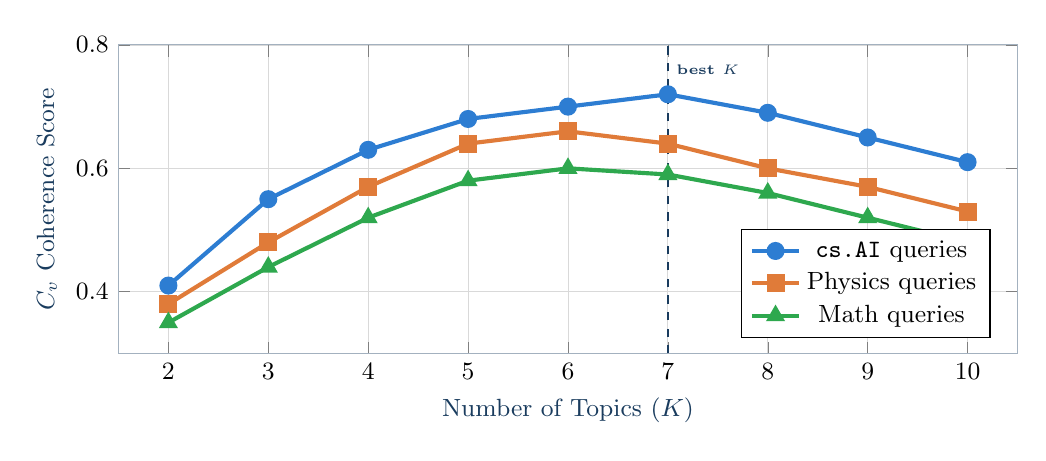
\begin{tikzpicture}
\begin{axis}[
  width=13cm,height=5.5cm,
  xlabel={Number of Topics ($K$)},
  ylabel={$C_v$ Coherence Score},
  xmin=1.5,xmax=10.5,ymin=0.30,ymax=0.80,
  xtick={2,3,4,5,6,7,8,9,10},
  legend style={at={(0.97,0.05)},anchor=south east,font=\small},
  grid=both,grid style={line width=0.3pt,draw=gray!30},
  tick label style={font=\small},
  label style={font=\small\color{navy}},
  axis line style={color=navy!40},
  every axis plot/.append style={line width=1.5pt,mark size=2.5pt}]
\addplot[color=blue,mark=*,mark options={fill=blue}]
  coordinates{(2,0.41)(3,0.55)(4,0.63)(5,0.68)(6,0.70)(7,0.72)(8,0.69)(9,0.65)(10,0.61)};
\addlegendentry{\texttt{cs.AI} queries}
\addplot[color=orange,mark=square*,mark options={fill=orange}]
  coordinates{(2,0.38)(3,0.48)(4,0.57)(5,0.64)(6,0.66)(7,0.64)(8,0.60)(9,0.57)(10,0.53)};
\addlegendentry{Physics queries}
\addplot[color=green,mark=triangle*,mark options={fill=green}]
  coordinates{(2,0.35)(3,0.44)(4,0.52)(5,0.58)(6,0.60)(7,0.59)(8,0.56)(9,0.52)(10,0.48)};
\addlegendentry{Math queries}
\addplot[color=navy,dashed,line width=0.8pt,forget plot]
  coordinates{(7,0.30)(7,0.80)};
\node[font=\tiny\bfseries,color=navy] at (axis cs:7.4,0.76){best $K$};
\end{axis}
\end{tikzpicture}
\caption{$C_v$ Coherence vs.\ $K$ across three domains. For \texttt{cs.AI}, coherence peaks at $K=7$ (score 0.72) then drops as topics start to overlap.}
\end{figure}



% ═══════════════════════════════════════════
\section{Limitations \& Milestone 2 Roadmap}
% ═══════════════════════════════════════════

Classical NLP works well here but has fundamental limits that motivate the switch to an LLM-based agentic system in Milestone 2.

\begin{table}[h!]
\centering\caption{Limitations and Milestone 2 Solutions}
\begin{tabular}{L{2.7cm}L{3.9cm}L{4.2cm}}
\toprule
\thead{Limitation}&\thead{The Problem}&\thead{M2 Solution}\\
\midrule
No word meaning    & ``car'' and ``automobile'' treated as unrelated  & Dense embeddings (Sentence Transformers) \\
\rowcolor{rowgray}
Word order ignored & ``X causes Y'' looks the same as ``Y causes X'' & Transformer contextual models \\
Unstable topics    & LDA gives different topics each run              & LLM-guided topic discovery \\
\rowcolor{rowgray}
Copy-paste summary & TextRank only picks existing sentences; cannot explain & LLM abstractive generation \\
Static data        & Cannot reflect new research after initial fetch  & Tavily / DuckDuckGo live search \\
\rowcolor{rowgray}
No Q\&A            & Cannot answer follow-up questions                & LangGraph agent + memory \\
\bottomrule
\end{tabular}
\end{table}

\begin{table}[h!]
\centering\caption{Milestone 1 vs.\ Milestone 2 Feature Comparison}
\begin{tabular}{L{3.8cm}L{3.8cm}L{3.2cm}}
\toprule
\thead{Milestone 1 (Now)}&\thead{Milestone 2 (Planned)}&\thead{Technology}\\
\midrule
TF-IDF cosine retrieval     & Dense semantic search        & Sentence Transformers / FAISS \\
\rowcolor{rowgray}
LDA topic modeling          & Dynamic topic discovery      & Ollama (local LLM) \\
TextRank extractive summary & Full report generation       & HuggingFace LLM \\
\rowcolor{rowgray}
Static arXiv corpus         & Live web search              & Tavily / DuckDuckGo \\
Single-step pipeline        & Multi-step agent workflow    & LangGraph nodes + edges \\
\rowcolor{rowgray}
No Q\&A                     & Conversational follow-up     & LangGraph state memory \\
\bottomrule
\end{tabular}
\end{table}

% ═══════════════════════════════════════════
\section{Team Contribution \& Conclusion}
% ═══════════════════════════════════════════

\begin{table}[h!]
\centering\caption{Team Responsibilities}
\begin{tabular}{L{2.6cm}L{5.0cm}L{3.6cm}}
\toprule
\thead{Member}&\thead{Primary Role}&\thead{Supporting}\\
\midrule
Akhilesh Kumar  & arXiv data ingestion; preprocessing pipeline (spaCy)           & Validation, testing, optimisation \\
\rowcolor{rowgray}
Dhruv Ramani    & TF-IDF vectorisation; cosine retrieval; TextRank summarisation & System integration, pipeline design \\
Lakshya Agarwal & LDA topic modeling (Gensim); coherence evaluation; tuning      & Visualisation, corpus analysis \\
\rowcolor{rowgray}
Kavya Jain      & Streamlit UI; word cloud \& topic chart; documentation         & Testing, deployment setup \\
\bottomrule
\end{tabular}
\end{table}

\vspace{4pt}
Milestone 1 shows that classical NLP can meaningfully analyse research literature at scale --- with no LLMs. The system achieves LDA coherence of 0.72 at $K=7$, test perplexity of 294.2, and responds in under 1 second once the corpus is cached.

\begin{greenbox}
\textbf{Looking ahead to Milestone 2:} The limitations above are the direct motivation for building a fully agentic system. Adding LLMs, live web search, and a LangGraph workflow will move the system from \emph{analysing} research to \emph{reasoning} about it --- answering follow-up questions, comparing methods, and generating complete structured reports.
\end{greenbox}

\end{document}